\section{Øvelse 2}
\subsection{Opgave 1 - Half-adder}
\begin{enumerate}
	\item[1)]
	Architecture body i VHDL kan skrives på tre forskellige måder; dataflow, behavioral og structural. \\
	Half-adder beskrives i Dataflow style ved hjælp af direkte implementering af logiske gates. Skrivemåden gør det nemt at overføre programmet direkte til hardware og de logiske gates. \\
	I Behavioral style opskrives half-adderen ved brug af if/else statements. Dette giver en god forståelse af selve half-adderens funktion, men det er kompliceret at overføre det til logiske gates ud fra kodens syntax. \\
	I structural style laves et miks af de to ovenstående, da der først defineres en funktion for hver logisk gate som det ses i dataflow style, og derefter implementeres funktionerne i halfadder entity’en. Denne style er god at bruge, hvis man skal implementere en funktion flere gange.\\
	\item[2)]
	Et RTL view af de tre forskellige måder at skrive en half-adder på, giver følgende forskellige resultater:\\
\begin{figure}[h]
	\centering
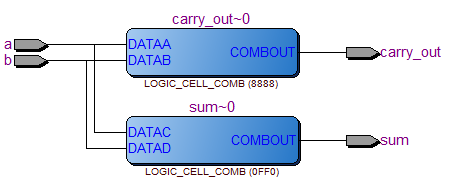
\includegraphics[scale=0.8]{pictures/Oevelse1/Half_adder/Behavioral.JPG}
\caption{Half-adder - Behavioral RTL view}
\label{fig:HaBehavioralRTL}
\end{figure}

\begin{figure}[h]
	\centering
	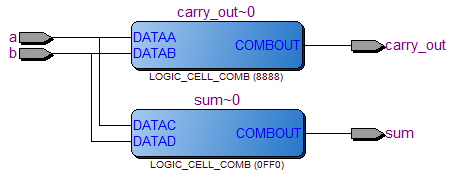
\includegraphics[scale=0.8]{pictures/Oevelse1/Half_adder/dataflow.JPG}
	\caption{Half-adder - Dataflow RTL view}
	\label{fig:HaDataflowRTL}
\end{figure}

\begin{figure}[h]
	\centering
	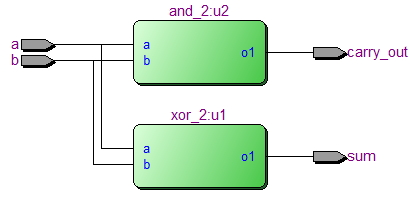
\includegraphics[scale=0.8]{pictures/Oevelse1/Half_adder/Structural.JPG}
	\caption{Half-adder - Structural RTL view}
	\label{fig:HaStructuralRTL}
\end{figure}
	\newpage
	
	Ud fra ovenstående figurer ses det, at dataflow-style og behavioral-style "afkodes" på samme vis, hvor de blå bokse symboliserer en logisk funktion. I structural-style angiver de grønne bokse, også logiske funktioner, men disse er defineret af os, som hhv en AND-funktion og en XOR-funktion. Det er altså med structural-style at vi nemmest kan se, hvilke gates vi skal bruge i en fysisk opbygning af systemet.\\

	\item[3)]
	Følgende tre figurer viser en Timing simulation af hver style. \\
\begin{figure}[h]
	\centering
	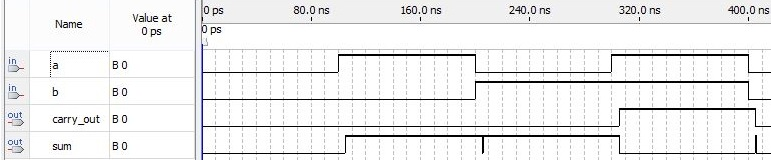
\includegraphics[scale=0.6]{pictures/Oevelse1/Half_adder/Behavioral_timing_simulation.jpg}
	\caption{Half-adder - Behavioral Timing Simulation}
	\label{fig:HaBehavioralTimingSim}
\end{figure}
\begin{figure}[h]
	\centering
	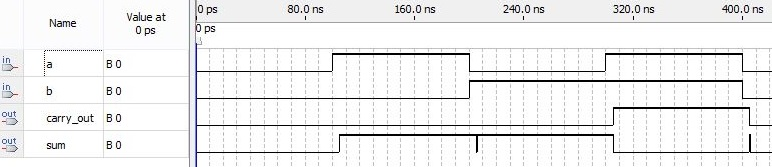
\includegraphics[scale=0.6]{pictures/Oevelse1/Half_adder/Dataflow_timing_simulation.jpg}
	\caption{Half-adder - Dataflow Timing Simulation}
	\label{fig:HaDatalfowTimingSim}
\end{figure}
\begin{figure}[h]
	\centering
	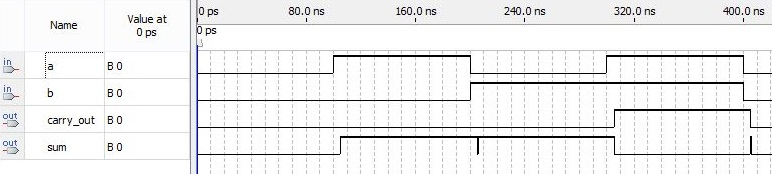
\includegraphics[scale=0.6]{pictures/Oevelse1/Half_adder/Structural_timing_simulation.jpg}
	\caption{Half-adder - Structural Timing Simulation}
	\label{fig:HaStructuralTimingSim}
\end{figure}
	\newpage
	Som det ses på figurerne, forekommer der nogle spikes på funktionerne. Dette skyldes static hazard, da de "gates" vi bruger i vores half-adder, vil have en lille tidsforskydning fra hinanden, og dermed kan give forkerte resultater i brøkdelen af et nanosekund, som det eksempelvis ses når både a-signalet og b-signalet ændrer status.
	\item[4)] 
	For at undgå disse spikes laver vi en functional simulation. Denne slags simulering tager højde for static hazard, og optimerer diagrammet til at vise et "perfekt" resultat.\\
	Figur \ref{fig:HaDataflowFunctionalSim}, \ref{fig:HaBehavioralFunctionalSim} og \ref{fig:HaStructuralFunctionalSim} viser denne type simulering.\\
\begin{figure}[h]
	\includegraphics[scale=0.6]{pictures/Oevelse1/Half_adder/Dataflow_functional_simulation.jpg}
	\caption{Half-adder - Dataflow functional Simulation}
	\label{fig:HaDataflowFunctionalSim}
\end{figure}
\begin{figure}[h]
	\includegraphics[scale=0.6]{pictures/Oevelse1/Half_adder/Behavioral_functional_simulation.jpg}
	\caption{Half-adder - Behavioral functional Simulation}
	\label{fig:HaBehavioralFunctionalSim}
\end{figure}
\begin{figure}[h]
	\includegraphics[scale=0.6]{pictures/Oevelse1/Half_adder/Structural_functional_simulation.jpg}
	\caption{Half-adder - Structural functional Simulation}
	\label{fig:HaStructuralFunctionalSim}
\end{figure}
	\newpage
\end{enumerate}

\subsection{Opgave 2 - Full-adder}
	\flushleft
\begin{enumerate}
	\item[1)]
	Med to half-addere kan man lave en full-adder. Dette vil vi nu implementere i hhv. dataflow-style, behavioral-style og structural-style.\\
	\medskip
	\begin{lstlisting}[caption={Full-adder Dataflow VHDL kode},label={lst:FaDataflowCode}]
	library ieee;
	use ieee.std_logic_1164.all;
	
	entity full_adder_dataflow is
	port (a, b, carry_in : in std_logic;
	sum, carry_out : out std_logic);
	end full_adder_dataflow;
	
	architecture dataflow of full_adder_dataflow is
	
	signal s1, s2, s3 : std_logic;
	begin
	s1 <= a xor b; 
	sum <= s1 xor carry_in;
	s2 <= s1 and carry_in;
	s3 <= a and b;
	carry_out <= s2 or s3;
	
	end dataflow;
	\end{lstlisting}
	\medskip
	\begin{lstlisting}[caption={Full-adder Behavioral VHDL kode}, label={lst:FaBehavioralCode}]
	library ieee;
	use ieee.std_logic_1164.all;
	
	entity full_adder_behavioral is
	port (a, b, carry_in : in std_logic;
	sum, carry_out : out std_logic);
	end full_adder_behavioral;
	
	architecture behavioral of full_adder_behavioral is
	
	signal s1, s2, s3 : std_logic;
	begin
	fa: process (carry_in, a, b)
	begin
	if carry_in = '0'  then
	
	if a = '1' then
	sum <= not b;
	carry_out <= b;
	else
	sum <= b;
	carry_out <= '0';
	end if;
	else 
	sum <= a xnor b;
	carry_out <= a or b;
	end if;
	end process fa;
	
	end behavioral;
	\end{lstlisting}
	\medskip
	\begin{lstlisting}[caption={Full-adder Structural VHDL kode},label={lst:FaStructuralCode}]
	library ieee;
	use ieee.std_logic_1164.all;
	
	entity full_adder_structural is
	port (a, b, carry_in : in std_logic;
	sum, carry_out : out std_logic);
	end full_adder_structural;
	
	architecture structural of full_adder_structural is
	
	signal s1, s2, s3 : std_logic;
	begin
	
	ha1: entity work.half_adder_dataflow port map (a => a, b => b, sum => s1, carry_out => s3);
	ha2: entity work.half_adder_dataflow port map (a => s1, b => carry_in, sum => sum, carry_out => s2);
	or1: entity work.or_2 port map (i1 => s2, i2 => s3, o1 => carry_out);
	
	end structural;
	\end{lstlisting}
	\newpage
	\flushleft
		\item[2)]
		Med et RTL view kan vi se hvordan de tre forskellige koder vil blive omdannet til logiske gates.\\
		\begin{figure}[h]
		\centering
		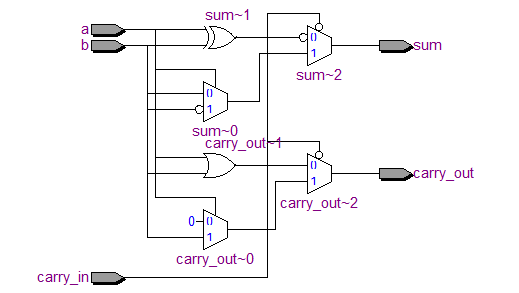
\includegraphics[scale=0.7]{pictures/Oevelse1/Full_adder/Behavioral_RTL.JPG}
		\caption{Full-adder - Behavioral RTL view}
		\label{fig:FaBehavioralRTL}
	\end{figure}
	
	\begin{figure}[h]
		\centering
		\includegraphics[scale=0.7]{pictures/Oevelse1/Full_adder/dataflow_RTL.JPG}
		\caption{Full-adder - Dataflow RTL view}
		\label{fig:FaDataflowRTL}	
	\end{figure}
	
	\begin{figure}[h]
		\centering
		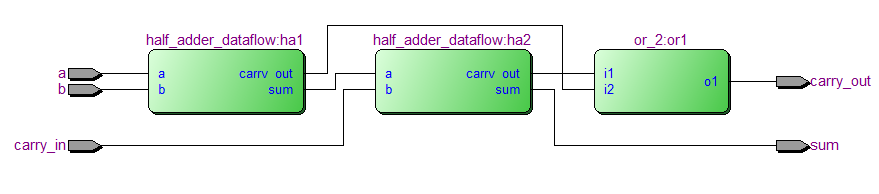
\includegraphics[scale=0.7]{pictures/Oevelse1/Full_adder/Structural_RTL.JPG}
		\caption{Full-adder - Structural RTL view}
		\label{fig:FaStructuralRTL}	
	\end{figure}
	
	\newpage
	\flushleft
		\item[3)]
		Til sidst laver vi en functional simulering for at se om vores tre full-adder koder opfører sig som vi ønsker.\\	

	\begin{figure}[h]
		\centering
		\includegraphics[scale=0.8]{pictures/Oevelse1/Full_adder/Dataflow_functional_simulation.jpg}
		\caption{Full-adder - Dataflow functional Simulation}
		\label{fig:FaDataflowFunctionalSim}
	\end{figure}
	\begin{figure}[h]
		\centering
		\includegraphics[scale=0.8]{pictures/Oevelse1/Full_adder/Behavioral_functional_simulation.jpg}
		\caption{Full-adder - Behavioral functional Simulation}
		\label{fig:FaBehavioralFunctionalSim}
	\end{figure}
	\begin{figure}[h]
		\centering
		\includegraphics[scale=0.6]{pictures/Oevelse1/Full_adder/Structural_functional_simulation.jpg}
		\caption{Full-adder - Structural functional Simulation}
		\label{fig:FaStructuralFunctionalSim}
	\end{figure}
	\newpage

\end{enumerate}

